\documentclass[11pt]{article}
\usepackage{amsmath}
\usepackage{amsfonts, amssymb}
\usepackage{color}
\usepackage{tikz}
\usetikzlibrary{arrows, chains, positioning, quotes, shapes.geometric}

\newcommand{\SPzt}{\mathcal{S}_0(1)}

\newcommand{\SPz}{\mathcal{S}_0(0)}

\newcommand{\SPo}{\mathcal{S}_1(0)}

\newcommand{\SPot}{\mathcal{S}_1(1)}

\begin{document}

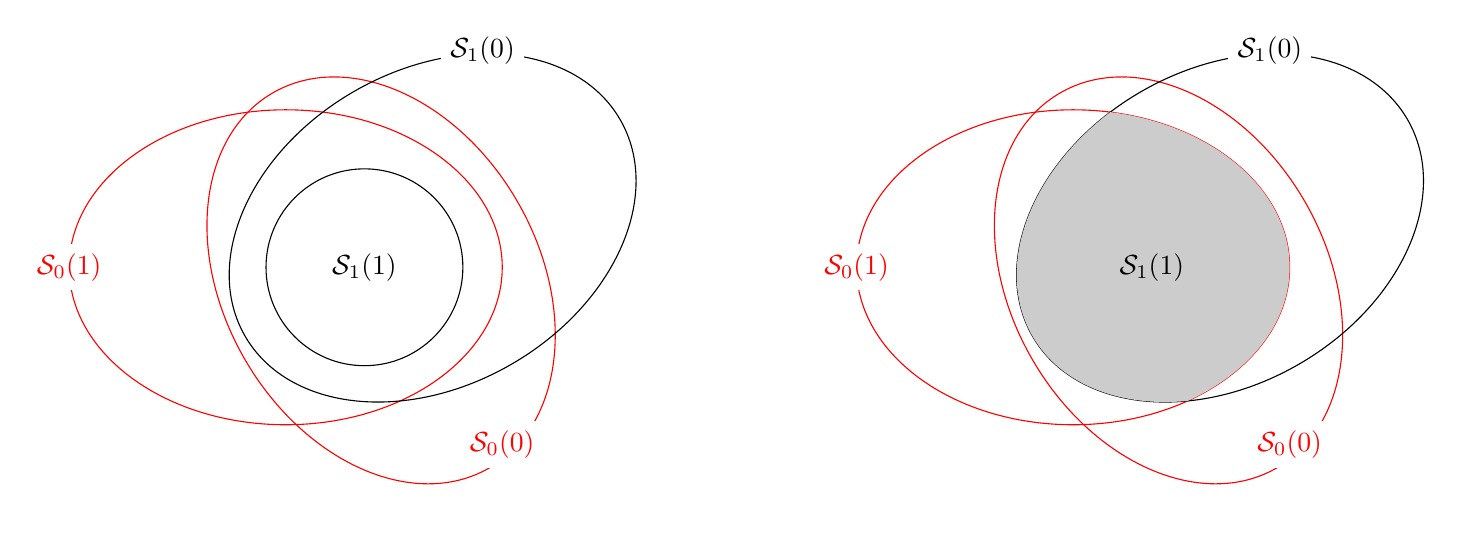
\begin{tikzpicture}[scale=1]
  \begin{scope}[fill opacity = 1,text opacity=1]
   \draw[rotate=300, color=red] (0.25,0.1) ellipse (2.75cm and 2cm);
   \draw[color=red] (-1,0) ellipse (2.75cm and 2cm);
   \draw[rotate=30] (1,0) ellipse (2.75cm and 2cm);
   \draw (0,0) circle[radius=1.25];
    \node[fill = white] at (-3.75, 0) (A) {{\color{red}$\SPzt$}};   
    \node[fill = white] at (1.75, -2.25) (B) {{\color{red}$\SPz$}};   
    \node[fill = white] at (1.5, 2.75) (C) {$\SPo$};   
    \node[fill = white] at (0, 0) (D) {$\SPot$};   
 
   \draw[rotate=300, color=red] (0.25+5,0.1+5*1.73205) ellipse (2.75cm and 2cm);
   \draw[color=red] (-1+10,0) ellipse (2.75cm and 2cm);
   \draw[rotate=30] (1+5*1.73205,0-5) ellipse (2.75cm and 2cm);
    \node[fill = white] at (-3.75+10, 0) (AA) {{\color{red}$\SPzt$}};   
    \node[fill = white] at (1.75+10, -2.25) (BB) {{\color{red}$\SPz$}};   
    \node[fill = white] at (1.5+10, 2.75) (CC) {$\SPo$};   
    \clip (-1+10,0) ellipse (2.75cm and 2cm);
    \clip[rotate=30] (1+5*1.73205,0-5) ellipse (2.75cm and 2cm);
    \fill[black!20!white] (8,-2) rectangle (12,2);
    \node[fill = none] at (0+10, 0) (DD) {$\SPot$};   
  \end{scope}
\end{tikzpicture}

\end{document}